% Généré par analysis/analyse.py -- ne pas modifier à la main.
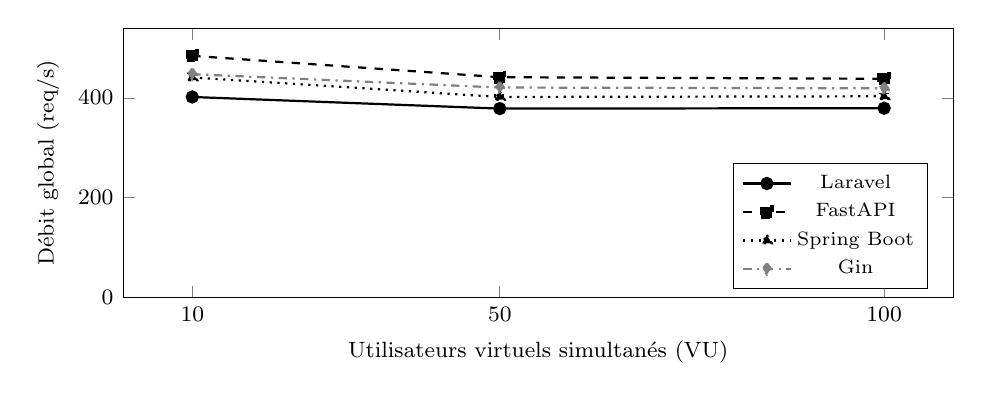
\begin{tikzpicture}
\begin{axis}[
  width=\columnwidth, height=5cm,
  xlabel={Utilisateurs virtuels simultanés (VU)},
  ylabel={Débit global (req/s)},
  xtick={10,50,100},
  tick label style={font=\footnotesize},
  label style={font=\footnotesize},
  legend style={font=\scriptsize, at={(0.97,0.03)}, anchor=south east},
  ymin=0]
\addplot[black, thick, mark=*, error bars/.cd, y dir=both, y explicit]
  coordinates {(10,401.73) +- (0,4.10) (50,378.43) +- (0,5.60) (100,379.28) +- (0,5.15)};
\addplot[black, thick, dashed, mark=square*, error bars/.cd, y dir=both, y explicit]
  coordinates {(10,484.20) +- (0,6.29) (50,441.36) +- (0,3.97) (100,438.18) +- (0,5.04)};
\addplot[black, thick, dotted, mark=triangle*, error bars/.cd, y dir=both, y explicit]
  coordinates {(10,440.96) +- (0,7.02) (50,401.75) +- (0,3.97) (100,403.09) +- (0,5.31)};
\addplot[gray, thick, dashdotted, mark=diamond*, error bars/.cd, y dir=both, y explicit]
  coordinates {(10,447.46) +- (0,3.34) (50,420.65) +- (0,2.46) (100,419.06) +- (0,3.26)};
\legend{Laravel, FastAPI, Spring Boot, Gin}
\end{axis}
\end{tikzpicture}
